% !Mode:: "TeX:UTF-8"

%%%% 此处是原创性声明的格式定义,数据填写的部分在下方 %%%

\makeatletter

\def\declaretitle#1{\def\@declaretitle{#1}}\def\@declaretitle{}
\def\declarecontent#1{\def\@declarecontent{#1}}\def\@declarecontent{}
\def\authorizationtitle#1{\def\@authorizationtitle{#1}}\def\@authorizationtitle{}
\def\authorizationcontent#1{\def\@authorizationcontent{#1}}\def\@authorizationconent{}
\def\authorizationadd#1{\def\@authorizationadd{#1}}\def\@authorizationadd{}
\def\authorsigncap#1{\def\@authorsigncap{#1}}\def\@authorsigncap{}
\def\supervisorsigncap#1{\def\@supervisorsigncap{#1}}\def\@supervisorsigncap{}
\def\signdatecap#1{\def\@signdatecap{#1}}\def\@signdatecap{}

% 定义makecopyright以生成原创性说明
\def\makecopyright{
	
	\clearpage
	
	% 如果需要上传稿包含版权页,取消这部分内容注释
	%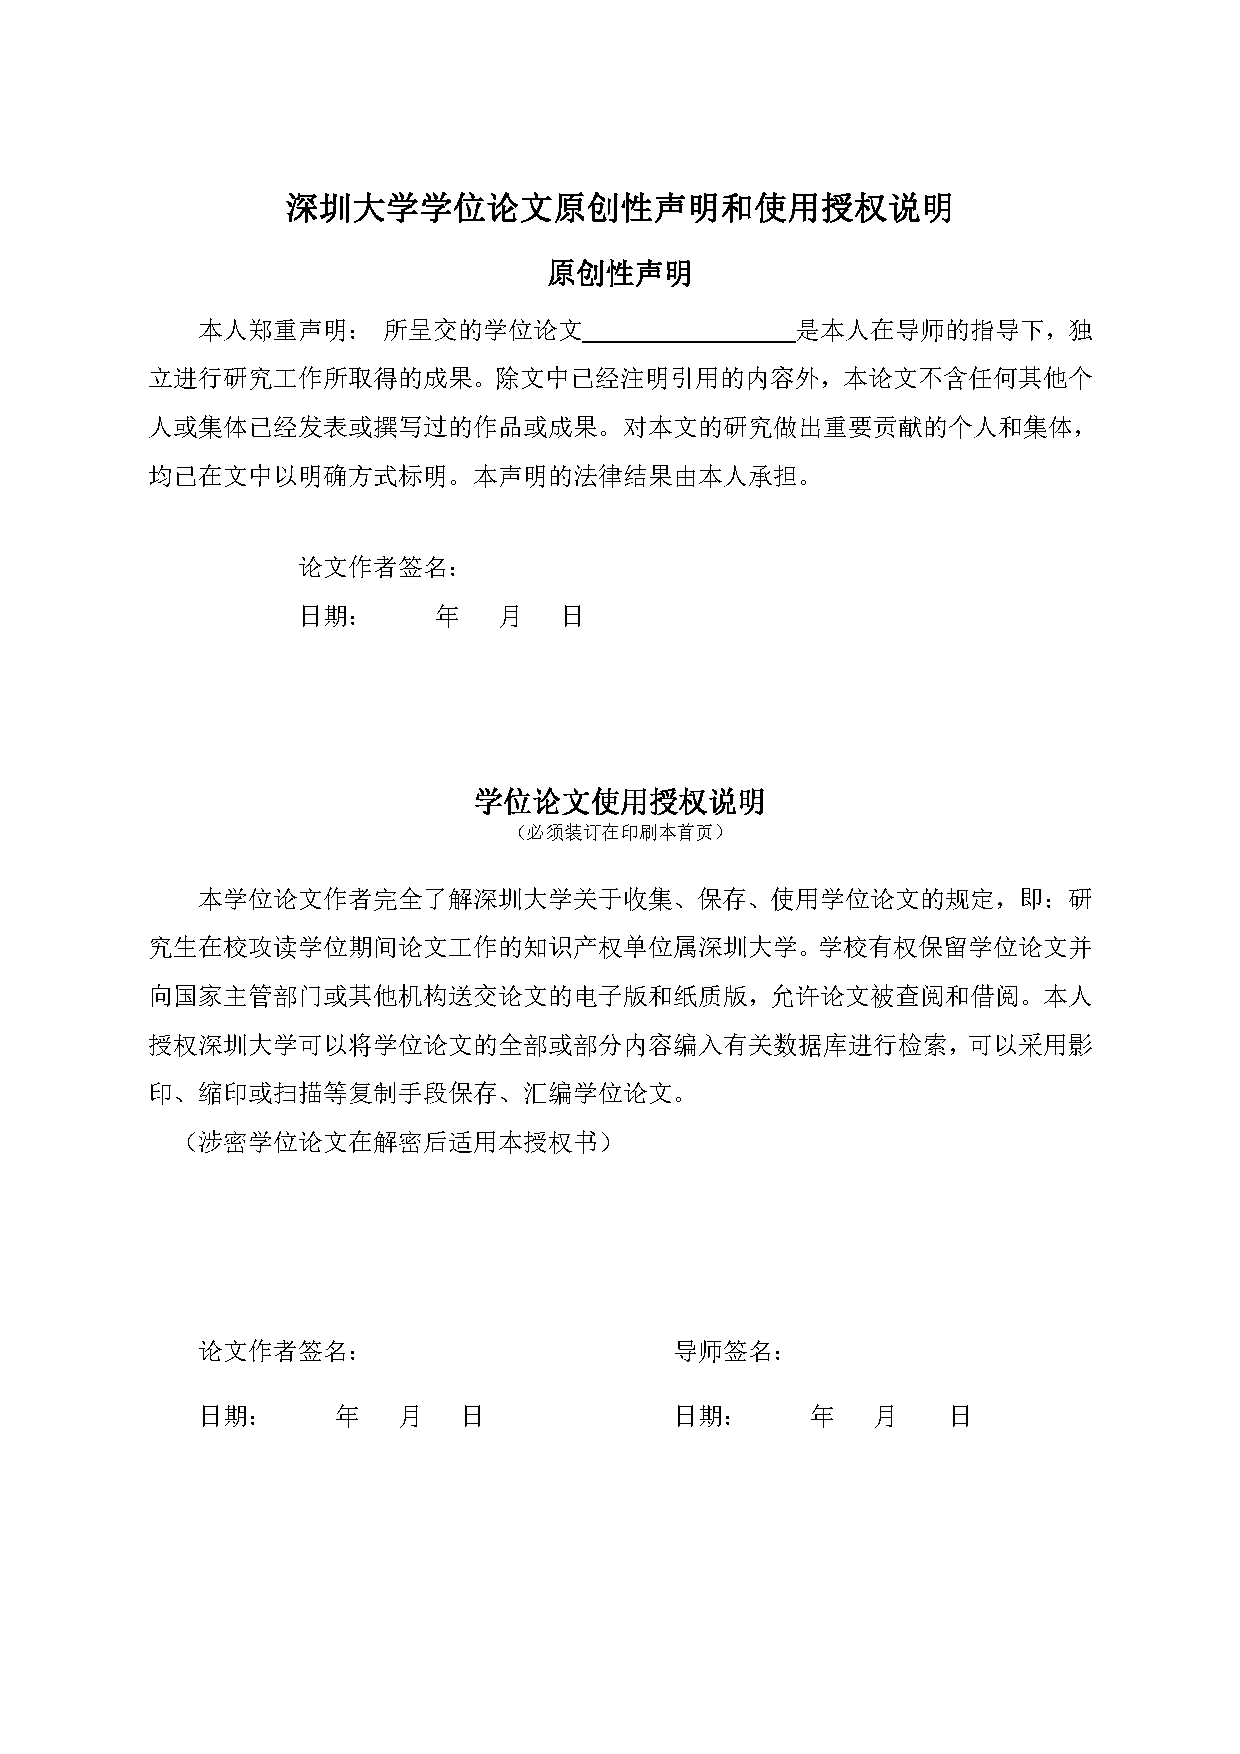
\includepdf{data/Copyright.pdf}
	
	
	% 下面的原创性声明页面的格式设置,如果引入pdf文件作为原创性声明,则将此部分代码注释掉
	\pagestyle{fancy}
	\fancyhf{}
	\fancyfoot[C]{\song\xiaowu ~\thepage~}
	\renewcommand{\headrulewidth}{0pt}
	\chapter*{\song\sanhao 深圳大学学位论文原创性声明和使用授权说明}{		% modified by Jon, 原创性说明无需加入目录,使用chapter*
		\thispagestyle{empty} 		% modified by Jon: 原创性说明不需要页码
		\qquad\\
		\begin{center}\hei\xiaoer{\@declaretitle}\end{center}\par
		\song\defaultfont{\@declarecontent}\par
		\vspace*{1cm}
		{\song\xiaosi
			\@authorsigncap \makebox[2.5cm][s]{}
			\@signdatecap \makebox[2cm][s]{} 年 \makebox[1cm][s]{} 月 \makebox[1cm][s]{} 日
		}
		\vspace{0.6\baselineskip}
		\begin{center}\hei\xiaoer{\@authorizationtitle}\end{center}\par
		{
			\vspace{1.2\baselineskip}
			\song\defaultfont{\@authorizationcontent}
			\par \song\defaultfont{\@authorizationadd}
		}
		\vspace{2\baselineskip}
		
		{
			\song\xiaosi
			\@authorsigncap \makebox[3.5cm][s]{}  \@signdatecap \makebox[1.5cm][s]{} 年 \makebox[1cm][s]{} 月 \makebox[1cm][s]{} 日 \\
			\indent
			\@supervisorsigncap \makebox[3.5cm][s]{}  \@signdatecap \makebox[1.5cm][s]{} 年 \makebox[1cm][s]{} 月 \makebox[1cm][s]{} 日
		}
	}
}
\makeatother

%%%% 数据填写的部分 %%%

\declaretitle{原创性声明}
\declarecontent{
	本人郑重声明: 所呈交的学位论文\underline{《xxx》}是本人在导师的指导下,独立进行研究工作所取得的成果。除文中已经注明引用的内容外,本论文不含任何其他个人或集体已经发表或撰写过的作品或成果。对本文的研究做出重要贡献的个人和集体,均已在文中以明确方式标明。本声明的法律结果由本人承担。
}
\authorizationtitle{学位论文版权使用授权书}
\authorizationcontent{
	本学位论文作者完全了解深圳大学关于收集、保存、使用学位论文的规定,即:研究生在校攻读学位期间论文工作的知识产权单位属深圳大学。学校有权保留学位论文并向国家主管部门或其他机构送交论文的电子版和纸质版,允许论文被查阅和借阅。本人授权深圳大学可以将学位论文的全部或部分内容编入有关数据库进行检索,可以采用影印、缩印或扫描等复制手段保存、汇编学位论文。
}
\authorizationadd{(涉密学位论文在解密后适用本授权书)}
\authorsigncap{作者签名:}
\supervisorsigncap{导师签名:}
\signdatecap{签字日期:}

% 使用makecopyright生成原创性说明
\makecopyright